\documentclass[12pt]{article}
\usepackage[utf8]{inputenc}
\usepackage[spanish]{babel}
\usepackage[margin=2.5cm]{geometry}
\usepackage{amsmath, amssymb}
\usepackage{graphicx}
\usepackage{float}
\usepackage{xcolor}
\usepackage{hyperref}

\title{\textbf{Activación en Redes Neuronales}}
\author{Vazquez Garcia Mauricio Alexis}
\begin{document}

\maketitle

\section*{En pocas palabras}
En este trabajo comparamos el comportamiento de tres funciones de activación en la capa oculta ($\text{Sigmoide}$, $\tanh$ y $\text{ReLU}$) aplicadas a dos problemas geométricos:
uno de clasificación binaria  y otro multiclase. Analizamos qué tan rápido entrenan, la estabilidad del aprendizaje y la forma gráfica de las fronteras encontradas.

\section{Respuestas al Cuestionario}

\subsection{a) ¿Qué modificaciones le hicimos al código?}
Para cambiar la función de activación en la capa oculta, hicimos los siguientes ajustes principales en los scripts de MATLAB:

\begin{itemize}
    \item \textbf{Nuevas funciones y sus derivadas:} Reemplazamos la sigmoide de la capa oculta declarando las nuevas operaciones y sus derivadas paso a paso:
    \begin{itemize}
        \item Para $\tanh$: usamos \texttt{tanh(z)} y su derivada respecto a la activación $a$: $(1 - a^2)$.
        \item Para $\text{ReLU}$: usamos \texttt{max(0, z)} y su derivada condicional $1$ si $a > 0$ o $0$ en caso contrario.
    \end{itemize}
    \item \textbf{Capa de Salida Intacta:} La capa de salida no se modificó: en la red binaria se conservó la $\text{Sigmoide}$ para obtener valores entre $0$ y $1$, mientras que en la red multiclase 
    se mantuvo la función $\text{Softmax}$ para representar probabilidades.
    \item \textbf{Medición de tiempo:} Agregamos las instrucciones \texttt{tic} al iniciar el entrenamiento y \texttt{toc} al terminar la última época o activarse la parada por paciencia.
\end{itemize}
\newpage 
\subsection{b) Comparación de Tiempos de Ejecución}
La función \textbf{ReLU} resultó ser la más rápida en ejecutar todas las épocas, seguida por la \textbf{Tangente Hiperbólica} y, por último, la \textbf{Sigmoide}.

\begin{table}[H]
\centering
\begin{tabular}{|l|c|c|}
\hline
\textbf{Función de Activación} & \textbf{Tiempo Binario Promedio} & \textbf{Tiempo Multiclase Promedio} \\ \hline
Sigmoide &  2.66 s & .33 s\\ \hline
Tangente Hiperbólica ($\tanh$) & 3.06 s & .33 s \\ \hline
\textbf{ReLU} & \textbf{2.66 s} & \textbf{.31 s} \\ \hline
\end{tabular}
\caption{Tiempos promedio de ejecución por corrida.}
\end{table}

\textbf{¿Por qué ocurre esto?\n }

\textbf{Costo matemático:} La sigmoide y la $\tanh$ usan operaciones exponenciales ($e^{-z}$), las cuales toman más trabajo de cálculo para el procesador. En cambio, $\text{ReLU}$ solo hace una comparación sencilla (\texttt{max(0, z)}).

\subsection{c) Resultados al correr el código 3 veces}
Al ejecutar cada versión 3 veces 
\begin{figure}[H]
    \centering
    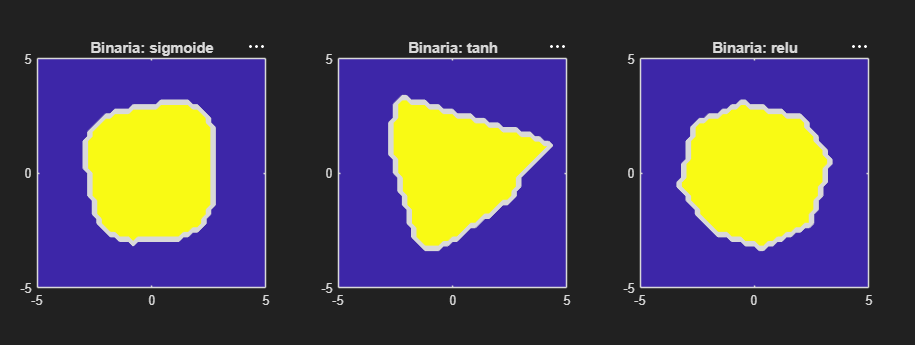
\includegraphics[width=0.8\textwidth]{bin.png}
    \caption{Resultados obtenidos al ejecutar el codigo.}
\end{figure}

\begin{figure}[H]
    \centering
    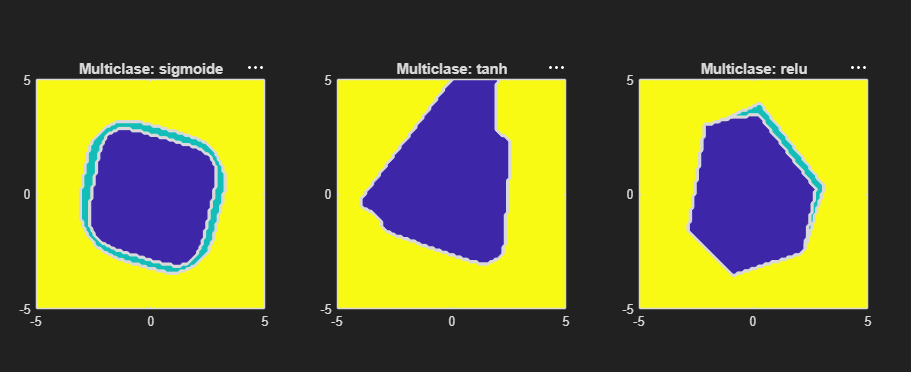
\includegraphics[width=0.8\textwidth]{multi.png}
    \caption{Resultados obtenidos al ejecutar el codigo.}
\end{figure}

\textbf{Observaciones clave:}
\begin{itemize}
    \item \textbf{Sigmoide:} Aprendió bastante rápido, pero son cuadrados con vertices redondeados.
    \item \textbf{Tangente Hiperbólica ($\tanh$):} Sus fronteras se ven más triangulares o con bordes rectos (fasetados) 
    \item \textbf{ReLU:} Fue la más estable. Dio las fronteras más redondas y suaves tanto para el círculo como para el aro.
\end{itemize}

\subsection{d) ¿Cuál fue la mejor función de activación y por qué?}
Para este tipo de problemas con fronteras de decisión redondas (curvas geométricas), la mejor opción general fue la \textbf{ReLU }).

\begin{table}[H]
\centering
\begin{tabular}{|l|c|c|c|}
\hline
\textbf{Criterio} & \textbf{Sigmoide} & \textbf{($\tanh$)} & \textbf{ReLU} \\ \hline
Velocidad & Rapida & Lenta & Muy Rápida \\ \hline
Frontera & Cuadrada & imprecisa & \textbf{Cuadrada casi esferica} \\ \hline
Estabilidad & Alta & Baja & \textbf{Media} \\ \hline
\end{tabular}
\caption{Resumen comparativo entre funciones.}
\end{table}

\textbf{Conclusión:} Aunque $\text{sigmoide}$ es imbatible en velocidad de cálculo, la ReLU logra curvas suaves con pocas neuronas en la capa oculta. La Tanh en la capa oculta no se recomienda debido a su lentitud y lo imprecisa en sus fronteras.

\end{document}